\section{Some Examples}

Let’s take a moment to examine some examples of the fascinating new graphs I obtained! Each will display a number of $N$ Units Away Curves next to one another.

\begin{figure}[h] 
  \label{example-1} 
  \begin{minipage}[b]{0.5\linewidth}
    \centering
    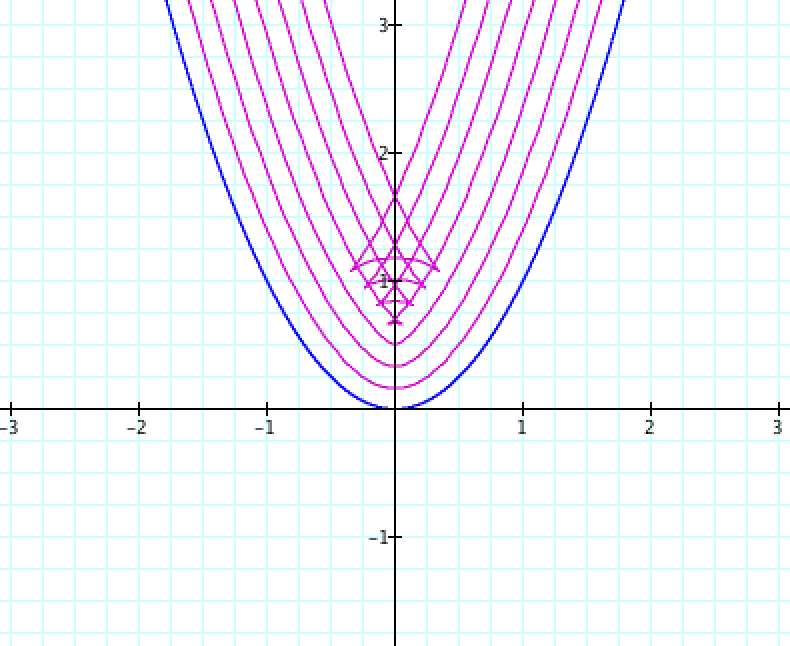
\includegraphics[width=.9\linewidth]{some-examples-img/Fig 5.png} 
    \caption{$f(x) = x ^ 2, N$ is positive} 
    \label{fig:fig5}
    \vspace{4ex}
  \end{minipage} % end 
  \begin{minipage}[b]{0.5\linewidth}
    \centering
    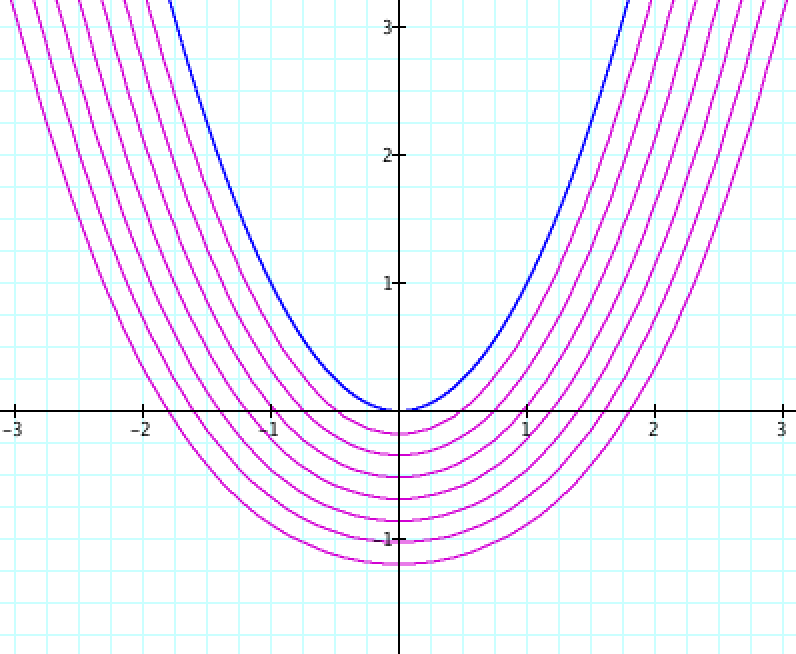
\includegraphics[width=.9\linewidth]{some-examples-img/Fig 6.png}
    \caption{$f(x) = x ^ 2, N$ is negative}
    \label{fig:fig6}
    \vspace{4ex}
  \end{minipage} % end
\end{figure}


\begin{figure}[h] 
  \label{example-2}
  \centering
  \begin{minipage}[b]{0.8\linewidth}
    \centering
    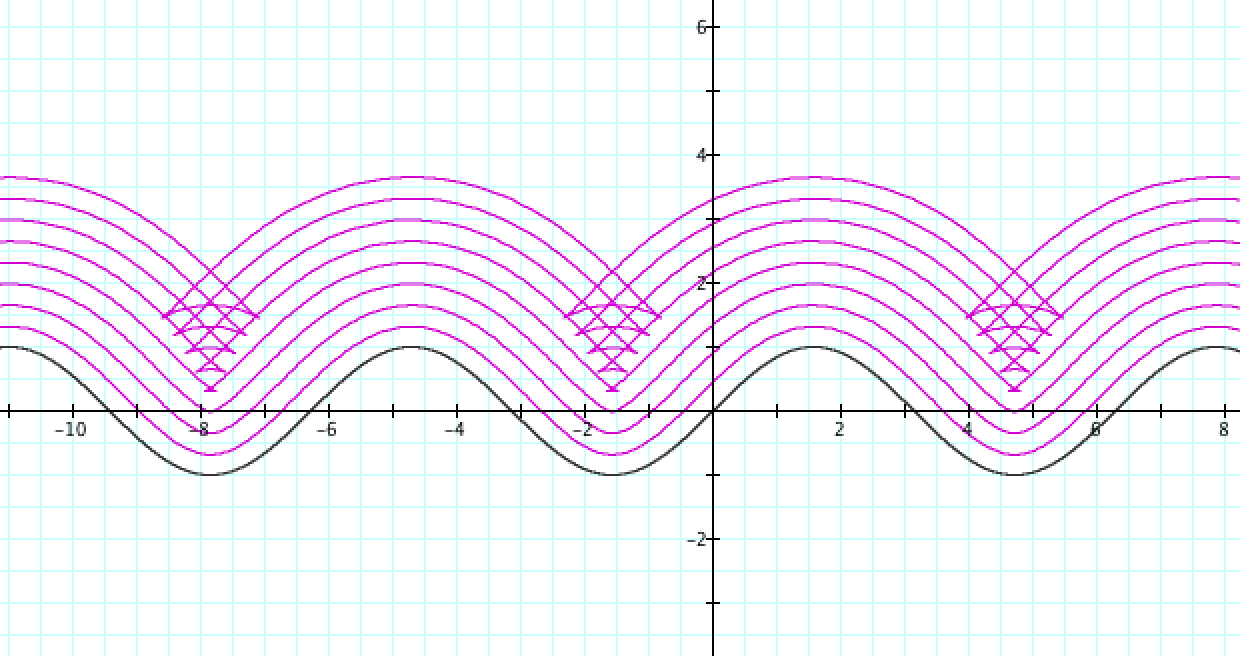
\includegraphics[width=.9\linewidth]{some-examples-img/Fig 7.png}
    \caption{$f(x) = sin x, N$ is positive}
    \label{fig:fig7}
    \vspace{4ex}
  \end{minipage} % end
\end{figure}

\begin{figure}[h] 
  \label{example-3}
  \begin{minipage}[b]{0.5\linewidth}
    \centering
    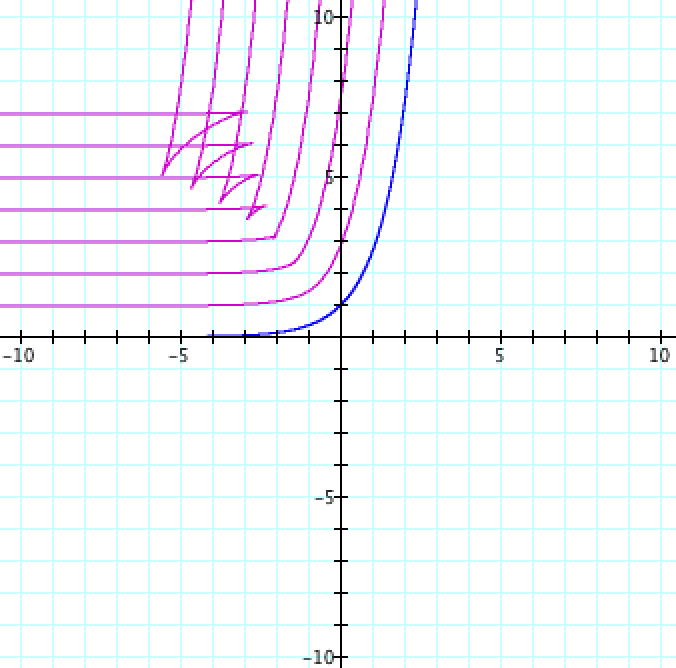
\includegraphics[width=.9\linewidth]{some-examples-img/Fig 8.png}
    \caption{$f(x) = e^x, N$ is positive}
    \label{fig:fig8}
    \vspace{4ex}
  \end{minipage} % end
  \begin{minipage}[b]{0.5\linewidth}
    \centering
    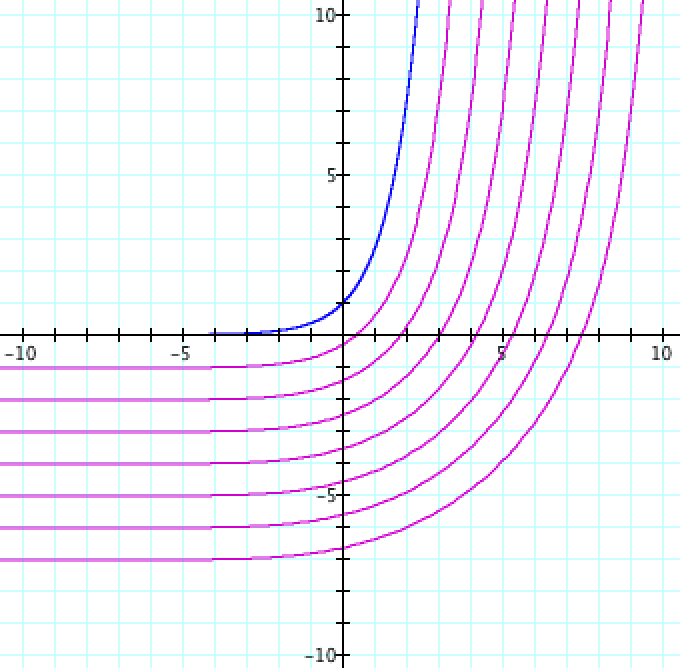
\includegraphics[width=.9\linewidth]{some-examples-img/Fig 9.png}
    \caption{$f(x) = e^x, N$ is negative}
    \label{fig:fig9}
    \vspace{4ex}
  \end{minipage} % end
\end{figure}

I loved these graphs! After so many years of drawing these things by hand, it was great to finally see them exactly and perfectly produced by computer. Playing with these $N$ Units Away Curves, I noted a few patterns very quickly.

\begin{itemize}
    \item The curves seem to stay smooth if you push them out opposite to the direction that the curve is bending.
    \item On the other hand, when you push the curves into the direction that the curve is bending, they seem to inevitably reach a critical value of $N$ and then ``crunch'' upon themselves, ceasing thereafter to pass the vertical line test and even be a function at all.
    \item When you produce these graphs, set $N$ to zero, and observe what happens as you gradually increase $N$... you find that for each region of the curve that has any bend to it, at some critical value of $N$ the $N$-Units Away Curves seem to collapse and crunch upon themselves at a unique ``crunch spot''. 
    \item Past that critical value, the $N$-Units Away Curves seem to thereafter generate a sort of odd-ball curvy triangle. These ``Divot Triangles'' were highly unexpected and I found them very intriguing. They always seemed to originate directly out of each crunch spot and grow from there. I noticed that as $N$ increases past the critical value, the divot triangle thus created swells and as it does so each of its vertices follows some particular path in $\mathbb{R}^2$. I found these ``divot paths'' fascinating and their logic mysterious. For example with the function $f(x) = x^3$, the top vertex of the triangle seems to follow a path that sweeps out to the left. Why in the world is that?
\end{itemize}

\begin{figure}[h!] 
  \label{example-4}
  \begin{minipage}[b]{0.5\linewidth}
    \centering
    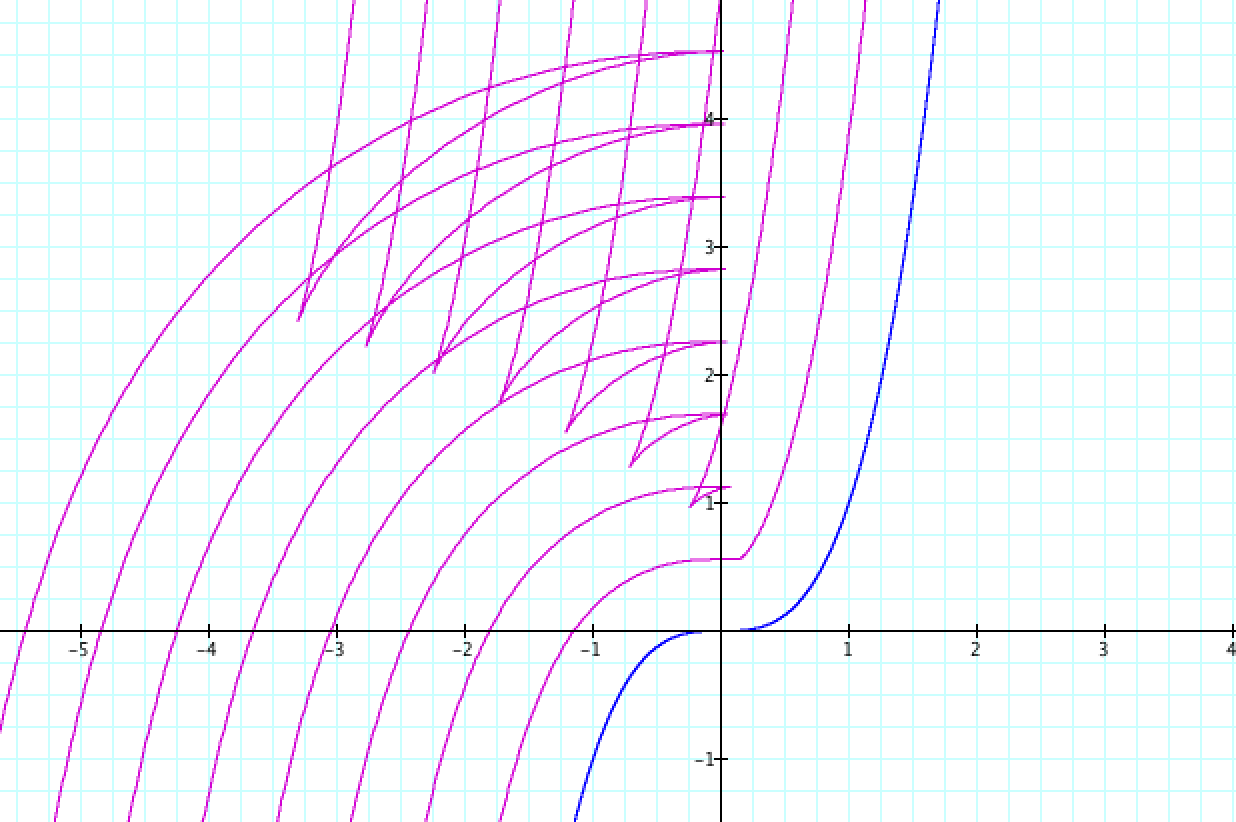
\includegraphics[width=.9\linewidth]{some-examples-img/Fig 10.png}
    \caption{$f(x) = x^3$, Divot Triangles}
    \label{fig:fig10}
    \vspace{4ex}
  \end{minipage} % end
  \begin{minipage}[b]{0.5\linewidth}
    \centering
    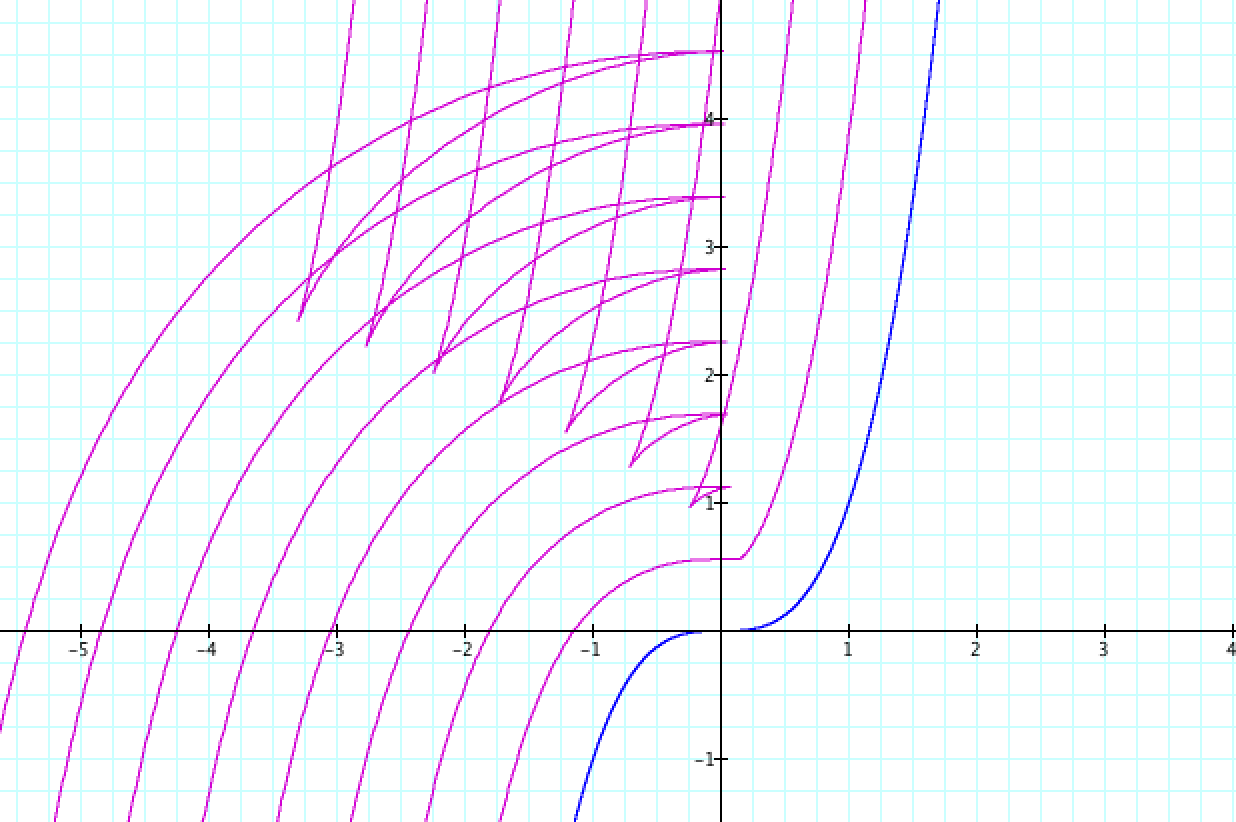
\includegraphics[width=.9\linewidth]{some-examples-img/Fig 11.png}
    \caption{$f(x) = x^3$, Divot Paths}
    \label{fig:fig11}
    \vspace{4ex}
  \end{minipage} % end
\end{figure}

\begin{figure}[h!] 
  \centering
  \label{example-5}
  \begin{minipage}[b]{0.8\linewidth}
    \centering
    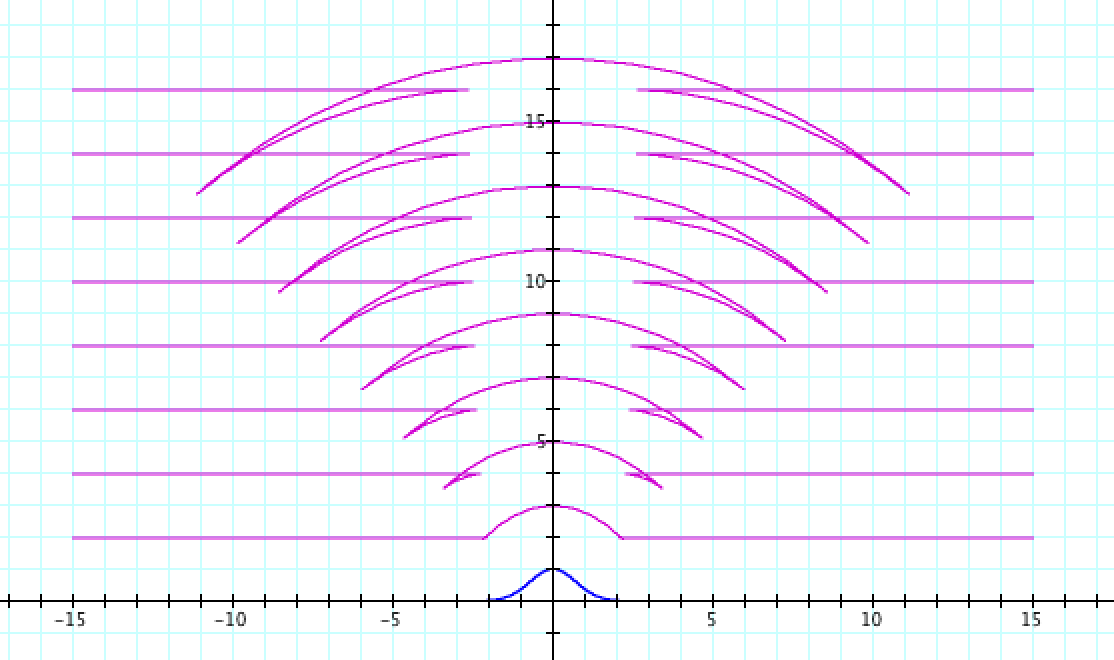
\includegraphics[width=.9\linewidth]{some-examples-img/Fig 12.png}
    \caption{$f(x) = e^{-x^2}$, Divot Paths}
    \label{fig:fig12}
    \vspace{4ex}
  \end{minipage} % end
\end{figure}

